\fancychapter{Introduction}
\label{cap:int}

\slshape

The isolation of graphene in 2004 has led to a growing interest of the scientific community in \ac{2D} materials revealing extraordinary properties.
Among them are \acp{TMD}, appearing in the form of a variety of nanostructures.
Unlike in graphene, where electron interactions are relatively weak, in \acp{TMD}, electrons are strongly correlated, and one cannot overlook the interactions between them.
Analytical approaches to the solution of the problem are either hopeless, or rely on possibly unrealistic approximations.
In fact, the increased complexity of the models describing such highly correlated  materials, compared to their graphene counterparts, calls for sophisticated computer simulation methods, most notably \ac{QMC}.
In this introductory chapter, we start by  reviewing the literature on the physics of \acp{TMD}, focusing on their basic properties.
Then, we present a survey of simulation methods belonging to the \acl{QMC} class.
We introduce some basic concepts, and motivate the choice of the particular used  method.
Finally, we summarize our original contributions, and outline the structure of the thesis.

\normalfont

\section{Motivation}
\label{sec:motivation}

It might seem surprising that \ac{2D} systems were not considered as a real possibility before the discovery of graphene since they are often idealized in thought experiments, for example when investigating toy models of more complex higher dimensional systems.
In fact, while thin film deposition on comparably thicker substrates was commonplace long before 2004, \ac{2D} layers were thought not to exist independently from their 3D base.
Their existence was not expected \emph{a priori} because at first sight they seem to violate the Mermin-Wagner-Hohenberg theorem \cite{mermin_absence_1966, coleman_there_1973, hohenberg_existence_1967}, a no-go theorem that forbids ordering below three dimensions at finite temperature\footnote{\ac{2D} materials can be stable because not all the conditions of Mermin-Wagner-Hohenberg theorem are verified, namely the condition of short-ranged interactions. In the particular case of graphene sheets, ripples appear, which implies that the material is not strictly \ac{2D}, and thus can be stabilized. The issue is subtle, and is beyond the scope of this work.}.
The discovery of graphene paved the way for the search for similarly stable \ac{2D} materials, and since it was isolated, a plethora of these has been discovered.
A vast set of open problems remains to be solved within the realm of the fascinating and counterintuitive properties of the now huge variety of existing \ac{2D} systems.
In particular, in some of these, the effect of electron interactions is non negligible, leading to emergent phenomena.
These are collective effects that emerge as a result of the interactions between the individual components of a system.
The properties of the system's components do not directly percolate up; instead, they shape the interactions that dictate the system's properties sometimes in rather unexpected ways, leading to unusual behavior.

Interacting electron systems are often tackled by carrying out computer simulations.
\ac{QMC} is a family of numerical methods that are  amply applicable to condensed matter physics problems, and that are particularly well suited to study strongly correlated electrons.
Despite the system size being constrained due to limited simulation time, reliable, accurate and unbiased solutions are provided to the otherwise intractable quantum many-body problem.
The class of \acs{QMC} algorithms that is used in this work was introduced in the 1980's in a series of seminal papers by Hirsch and \acl{BSS}\footnote{After whom the \ac{BSS} algorithm, on which we based the implementation used in this work, is named.} \cite{hirsch_discrete_1983, hirsch_monte_1982, blankenbecler_monte_1981, hirsch_two-dimensional_1985, hirsch_monte_1983, hirsch_stable_1988, hirsch_antiferromagnetism_1989}, but it saw a recent surge \cite{dumitrescu_superconductivity_2016, berg_monte_2018, beyl_revisiting_2018, chang_recent_2015, esterlis_breakdown_2018, mondaini_determinant_2012, meng_characterization_2014, kung_characterizing_2016, johnston_determinant_2013, rademaker_determinant_2013, ying_determinant_2014, scalettar_numerical_2007, zhou_quantum_2014} due to the increase in computational power, and algorithmic development.
As a result, the field is currently very active. 
Method optimization can prove crucial in applications to widely studied physical models of electron interactions.
In particular, recent computational and algorithmic developments opened the door to study both larger and lower temperature systems \cite{jiang_fast_2016, lee_parallelization_2010, chang_recent_2015, bai_stable_2011}.
In this work, an implementation of determinant \acs{QMC} based on the \ac{BSS} algorithm is used to simulate a \ac{TMD} zigzag-edged nanoribbon, a nanostructure made of this recent member of the \acs{2D} materials family.
Preliminary mean field studies show that this type of nanostructures have a tendency towards magnetism in graphene \cite{yazyev_emergence_2010}, which makes them good candidates for use in nanospintronics.
Our mean field calculations for \acp{TMD} show a similar trend, motivating our subsequent \acs{QMC} study, in an attempt to test how realistic the mean field predictions are.
\acs{QMC} is a complementary, more accurate, and unbiased approach that can shed light upon not only magnetic, but also  other phenomena, like the formation of charge density waves and superconductivity in the context of generic interacting electron models. Hence \acs{QMC} has acquired a far-reaching importance as a flexible, and accurate numerical tool.
\section{Strongly correlated electron systems}
\label{sec:strongly_correlated}

Condensed matter physics is concerned with the emergence of the properties of quantum materials from complexity.
The central concept within this approach is that of symmetry breaking.
When a phase transition occurs, a system is said to condense into a phase of lower symmetry.
A simple pictorial example is the transition from a gas to a solid.
Statistically, any point within a gas is equivalent, that is, on average, the surroundings of all points look similar.
Formally, the system is then said to be fully translationally invariant.
On the other hand, in a solid, a point is only equivalent to a discrete set of other points.
In fact, a simplified view of a solid consists of a periodic arrangement of atoms occupying the points of a lattice.
Any point on the lattice can be reached starting from any other point upon translation by a lattice vector.
Thus, a system that makes a transition from the gaseous to the solid state becomes invariant only under a discrete set of translations, rather than a continuous one. 

A framework that is commonly used to identify symmetry breaking is the \ac{LG} theory of phase transitions.
The theory gives a prescription to discover phase transitions.
More precisely, it gives criteria for a symmetry to become manifest.
Although this framework is very useful, it turns out that the search for order relies on symmetry ideas well beyond condensed matter.
Symmetry breaking gives rise to emergent phenomena.
The idea of emergence rests on a constructionist, rather than a reductionist hypothesis: that the behavior of the many does not trivially follow from the behavior of the few.
As P.W. Anderson puts it, \say{The ability to reduce everything to simple fundamental laws does not imply the ability to start from those laws and reconstruct the universe.} \cite{anderson_more_1972}

The broad scope of condensed matter comes from the sheer number of possibilities that the symmetry breaking approach affords.
For the specific case of the \acs{LG} theory, one can study the emergence of magnetism, superconductivity, or superfluidity, just to name a few.
However, as we shall see, sometimes the \acs{LG} theory fails to capture a system's behavior, and we must resort to other theories to identify these, or other eventual properties that might arise.
The \acl{LG} procedure can be summarized as follows: identify an order parameter reflecting the underlying symmetry of the system, and minimize the free energy in order to deduce conditions for the symmetry to become manifest, leading to a phase transition.
The drawback of this \emph{variational} approach is that it might be difficult to identify an order parameter in the first place.
Moreover, even if we do manage to find one, the usual procedure may be impossible to perform.
It can easily happen that the degree of complexity of the order parameter is simply too high.
Additionally, and perhaps more importantly, not all phase transitions can be described by the LG paradigm.

On the one hand, there are systems where a different kind of order arises.
A prominent example is that of fractional quantum Hall effect, where (rather surprisingly!) the \emph{quasi-particles} describing the excitations of the quantum Hall fluid carry \emph{fractions} of the electron charge.
There is an intimate connection between charge fractionalization and topology, which may be understood in terms of the properties of the Laughlin states describing the quantum Hall fluid. However, while it is tempting to try to characterize the latter in terms of the \acs{LG} paradigm, it must actually be regarded as a distinct type of matter, where \say{topological order} arises \cite{wen_topological_1990}.
%The proposal put forward by Wen \cite{wen_topological_1990} rests on characterizing quantum states by their ground state degeneracy, and investigating how they change under operations defined on specific manifolds. 

On the other hand, for the so called strongly correlated systems we shall focus on in this work, there are phenomena which emerge specifically due to the interacting nature of the problem.
They are elusive because a description in terms of the \acs{LG} paradigm does not yield a behavior consistent with what is observed empirically.
Instead, order emerges from the complexity created by the interactions among all the constituents.
The \acs{LG} theory fails because it ignores these interactions by disregarding fluctuations in the microscopic configuration of the system.
This approximation consists of reducing the complex interactions to an effective \emph{mean field}, which is normally determined self consistently.
Strongly correlated systems require an approach beyond mean field, which makes them both extremely interesting and notoriously difficult to tackle.
The mean field view fails to describe them because it considers each constituent to interact only with an external entity representing the interactions with all other constituents, underestimating collective behavior.
In fact, the failure of mean field theory is not limited to correlated systems, and its success in describing a given system depends, for example, on the dimensionality\footnote{Normally, there is an upper critical dimension $d_c$ above which mean field is exact. Below $d_c$, its predictions might be useful qualitatively, but not quantitatively.} and on the range of the particular type of interaction that is considered.

In many cases, mean field theory is too extreme an approximation.
Nonetheless, its occasional failure at capturing the whole of a system's properties does not deem it  useless.
Actually, it is quite the contrary.
Mean field is often used as a first approach to build an intuitive physical picture for the general properties and behavior of the system.
Of course, this is done while keeping in mind that the description it provides is intrinsically insufficient.
Clearly, to extract the features of a correlated system we must extend it to the fully interacting case.

Strongly correlated quantum matter is ubiquitous and is at the heart of today's most advanced electronic materials, namely organic conductors, high $T_c$ (cuprate) superconductors, colossal  magnetoresistance materials, and \say{heavy-fermion}\footnote{The quasi-particles describing excitations in these materials behave like much heavier electrons, hence the name.} compounds. 
Actually, the problem of strong correlations has now expanded beyond condensed matter physics. Quark-gluon plasmas, believed to have been formed just a few microseconds after the Big Bang, also belong to this class of systems.
Another example comes from atomic physics: ultracold atoms in optical lattices behave in a very similar way to correlated electrons.
In fact, the behavior is so similar that these systems are being used as \emph{de facto} quantum simulators of correlated electron systems \cite{quintanilla_strong-correlations_2009}.

A central piece in the understanding of correlated matter is the Hubbard model.
It was introduced to bridge a gap between metals and magnetic insulators, building on the earlier work of Mott.
The model is extremely simple.
Electrons hop from atom to atom on a lattice, paying an energy penalty when they occupy the same site.
This repulsive effect results in correlations beyond those that are always present due to the fermionic nature of the particles obeying the Pauli exclusion principle.
In the limit of weak repulsion, the electrons are nearly free, and the system behaves like a metal.
Otherwise, the electrons become localized at fixed atomic positions resulting in magnetic insulating behavior.
The model is simple to formulate, but already includes highly nontrivial  correlation effects between all electrons in the solid.
Thus, it is not surprising that an exact solution exists only in \acs{1D} \cite{lieb_absence_1968}, and higher dimensional versions are still being studied more than 50 years after the model appeared \cite{hubbard_electron_1963}.
\section{State of The Art}
\label{sec:int_state}

Solving the many-body problem remains one of the greatest challenges in physics.
Following the wealth of attempts at such pursuit, certain phenomena arising due to the strong interactions in quantum systems are explained in different theoretical frameworks, namely superconductivity, the Mott metal-insulator transition, and fractional quantum Hall effect.
All of these breakthroughs represented revolutions in their respective fields with significant scientific and technological impact.

Only in very limited cases does an actual analytical solution exist for the  Schr\"odinger equation for a system of interacting particles.
One must resort to sophisticated approximation methods to obtain  information about the role played by the competing interactions under various conditions in the aforementioned cases.
It is then natural that numerical methods have become prominent as a tool for extracting useful information about this type of systems.
\ac{QMC} is amongst the most accurate and extensively studied ones.

The idea of all \ac{QMC} methods is to reduce the interacting problem to solving a set of integrals, which can be evaluated numerically through a standard stochastic procedure.
These integrals are arrived at upon formulating the quantum many-body description of the system using the Schr\"odinger equation.
Hence the name \acl{QMC}, which is used to distinguish it from Classical Monte Carlo.
In the classical version, one measures thermal averages, while in the quantum version, one measures expectations of operators over the Hilbert space of the system, corresponding to physical observables that fluctuate with a dynamics given by the Schr\"odinger equation.

\subsection{Beyond graphene: TMD nanoribbons}

\ac{2D} materials have steadily been drawing the attention of the community since graphene was experimentally isolated from a graphite sample by mechanical exfoliation, yielding a system constituted by a single layer of atoms (Figure \ref{fig:graphene}, left).
Since then, numerous studies have been made due to the promising properties of these materials, and the interesting as-yet-unseen phenomena occurring within them, for example: unconventional quantum Hall effect, absence of localization, and electrons behaving like massless relativistic particles (Figure \ref{fig:graphene}, right), providing a bridge between condensed matter physics and quantum electrodynamics \cite{katsnelson_graphene:_2007}.

\begin{figure}[H]
\hspace{1cm}
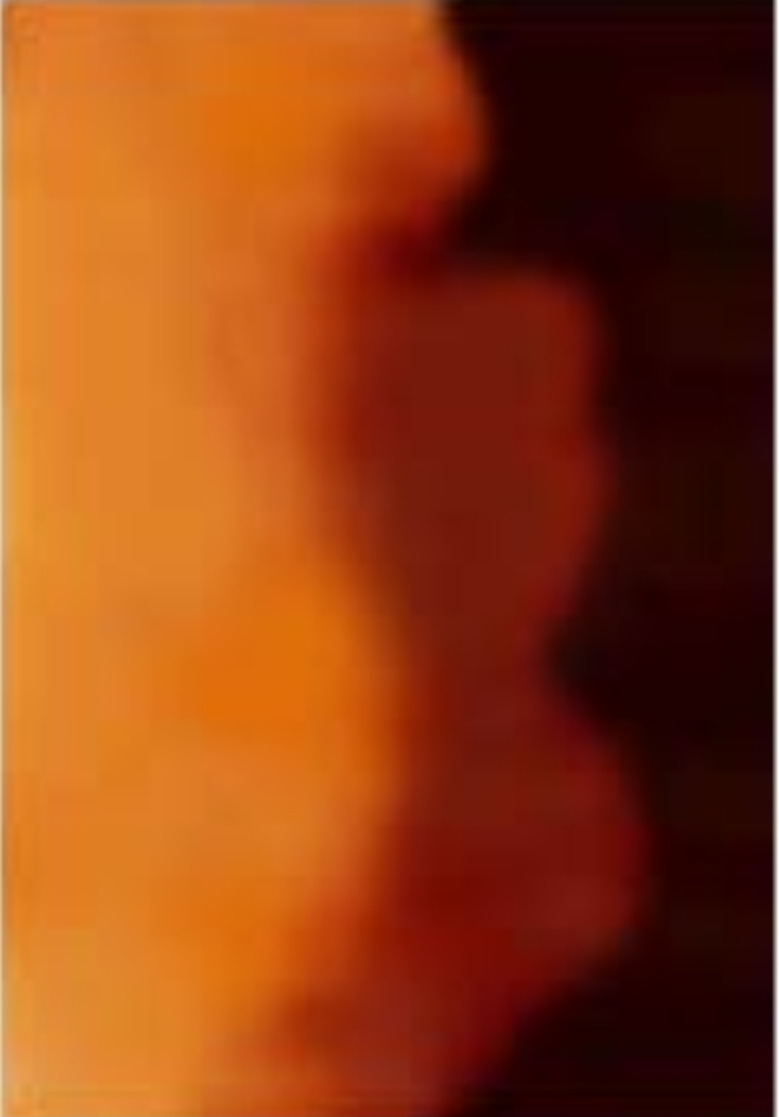
\includegraphics[width = 3.6cm]{Introduction/graphene.png}
\hspace{3cm}
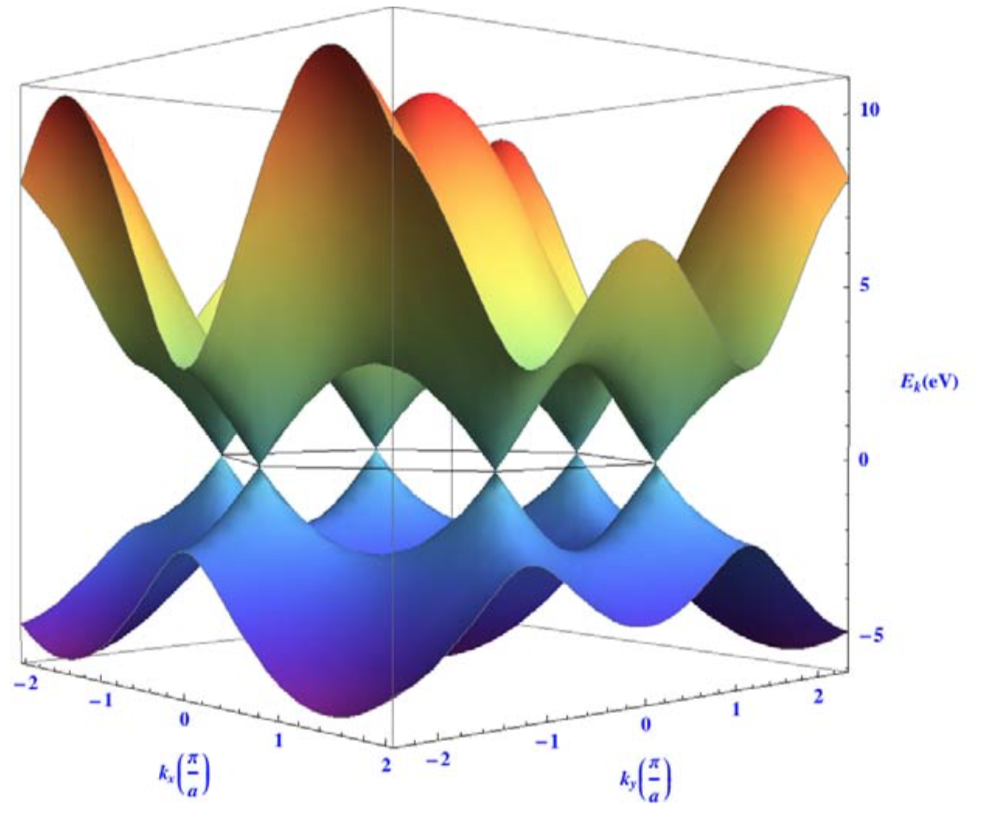
\includegraphics[width = 6.5cm]{Introduction/disp_rel.png}
\caption[Graphene monolayer; graphene's dispersion relation.]{Left: \acf{AFM} picture of a graphene monolayer. The black area is a substrate used for fabrication purposes. The dark orange area is a monolayer of graphene. Right: Dispersion relation of graphene. The black line represents the Fermi energy. Close to it, the dispersion relation is linear, corresponding to massless excitations (taken from \cite{noauthor_nobel_nodate}). }
\label{fig:graphene}
\end{figure}	

On the other hand, \acp{TMD} are a recent member of the \ac{2D} materials family \cite{wang_electronics_2012, roldan_electronic_2014, xu_spin_2014}.
\acp{TMD} have been attracting interest because they seem to overcome some of the drawbacks of graphene in technological applications.
For example, monolayer graphene is gapless, while its bilayer counterpart has only a tunable, but small gap of the order of a tenth of an $eV$.
Contrastingly, \acp{TMD} have an intrinsic gap in excess of $1 \, eV$, being more promising in designing, for example, transistors.
Hole-doped \acp{TMD} are expected to show topological superconductivity \cite{hsu_topological_2017}, while the superconducting phase of graphene has been predicted, but is not easily attained.
Superconductivity in graphene-like \ac{2D} materials is important because it could boost high speed nanoelectronics.
Moreover, the presence of transition metal atoms in \acp{TMD} suggests the possibility of magnetic ordering \cite{braz_valley_2017}, which could be very relevant in nanospintronics applications.
Both topological superconductivity and magnetic ordering arise due to the effect of strong electron correlations.
Thus, to investigate these properties of \acp{TMD} when performing simulations, we need a computational method that is robust enough to capture the effects of electron interactions.

A nanoribbon consists of a \ac{2D} layer that can be regarded as infinitely long on one direction, but not on the other (Figure \ref{fig:fabrication}), so that edge states become relevant, and can be controlled to yield interesting properties.
For simulation purposes, it is natural to assume translational invariance along the ribbon's longitudinal direction, and use \acp{PBC}.
On the other direction, we use \acp{OBC}, effectively considering zigzag edges (Figure \ref{fig:nanoribbons}, left).

\begin{figure}[H]
\centering
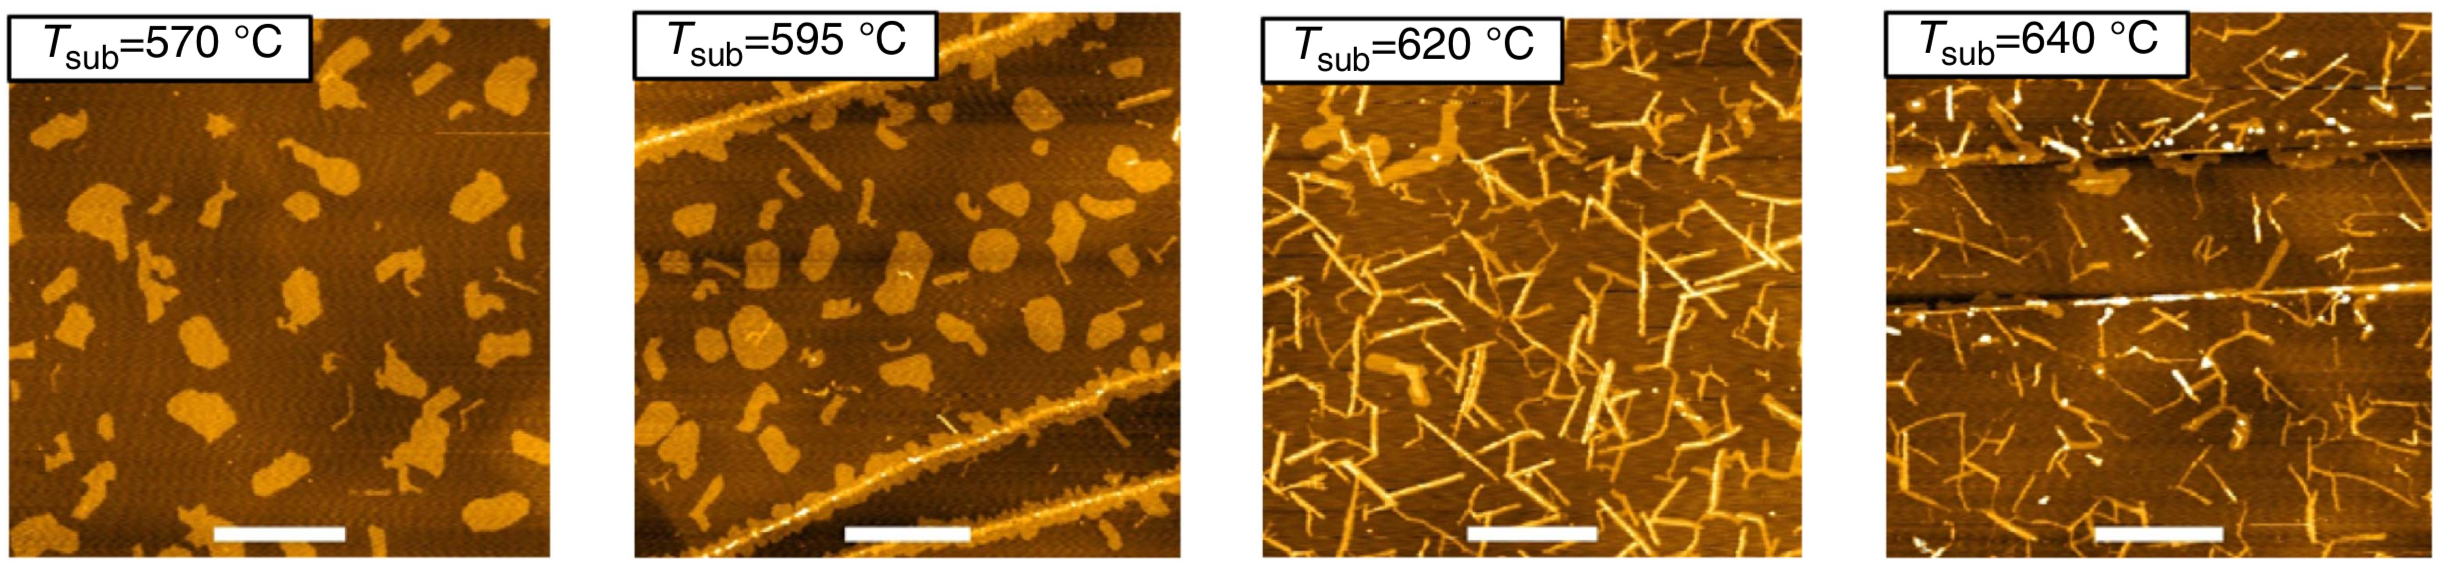
\includegraphics[scale = 0.35]{Introduction/nanoribbons}
\caption[Fabrication of \ac{TMD} nanoribbons]{Fabrication of \ac{TMD} nanoribbons. From left to right, we see \ac{AFM} images showing the appeareance of nanostructures ranging from \ac{2D} nanoislands to nanoribbons, as the temperature of the substrate is increased. The nanoribbons are grown by taking advantage of the temperature dependence of shape transformations occuring during the nonequilibrium growth of this kind of surface-based nanostructures. (taken from \cite{chen_fabrication_2017})}
\label{fig:fabrication}
\end{figure}
   
A high density of low-energy electronic states is localized at the zigzag edges, decaying quickly in the bulk, which suggests the possibility of magnetic ordering.
In fact, a mean field solution of the Hubbard model for a graphene nanoribbon shows that magnetic moments are localized at the edges \cite{yazyev_emergence_2010} (Figure \ref{fig:nanoribbons}, right).
QMC has been used to investigate edge-state magnetism beyond mean field in graphene \cite{feldner_dynamical_2011, golor_quantum_2013, cheng_strain-induced_2015, raczkowski_interplay_2017, yang_strain-tuning_2017}.
However, edge magnetism in TMD nanoribbons remains unexplored \cite{davelou_nanoribbon_2017}.
 
\begin{figure}[H]
\hspace{2cm}
\begin{minipage}[c]{0.1\textwidth}
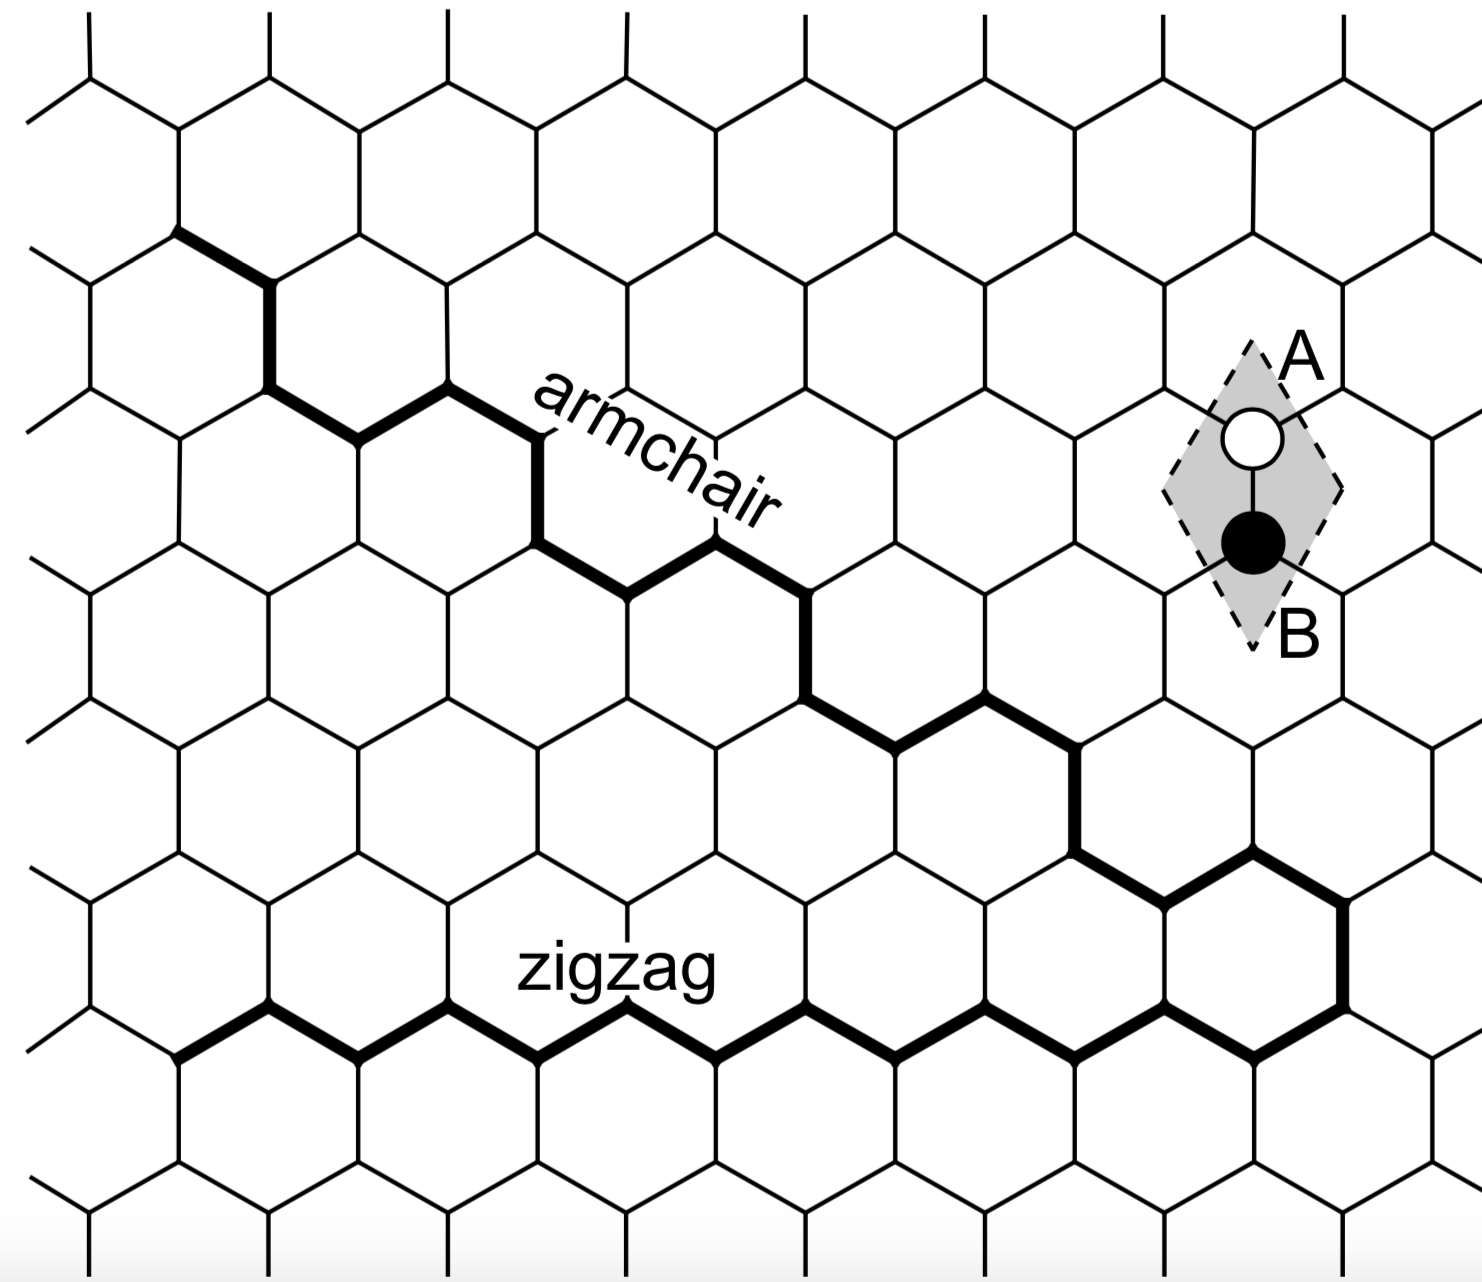
\includegraphics[scale = 0.22]{Introduction/zigzag}
\end{minipage} \hspace{6cm}
\begin{minipage}[c]{0.1\textwidth}
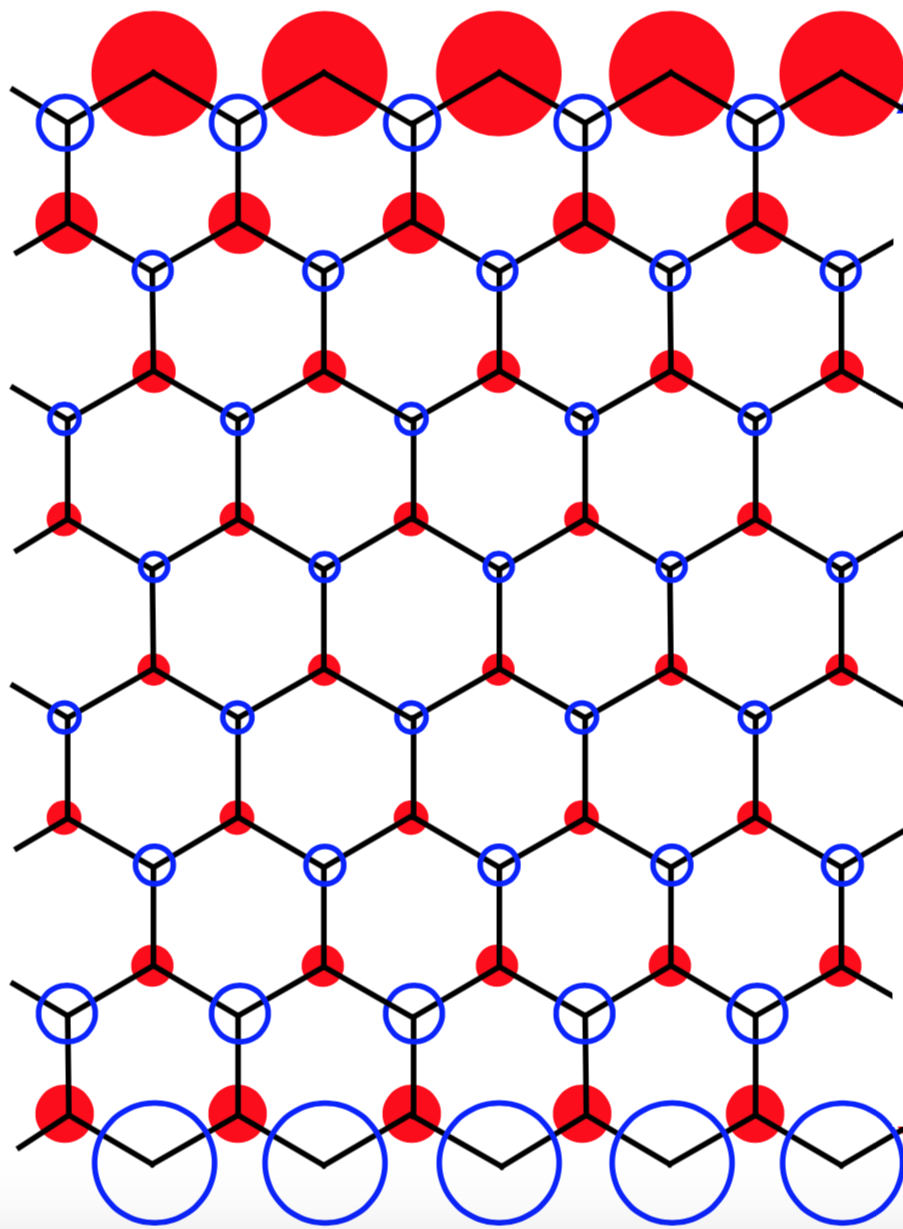
\includegraphics[scale = 0.23]{Introduction/edge_states}
\end{minipage}
 \caption[Zigzag edges of a nanoribbon and magnetism.]{Left: Two possible terminations of a \ac{TMD} nanoribbon condensing in a honeycomb lattice. Right: Local magnetic moments exist on the zig zag edges. The area of the circles corresponds to the magnitude of the magnetic moment, while the color red corresponds to a spin up density, and blue to a spin down density. The accumulation of electronic edge states leads to an \ac{AF} ground state (opposite edges with opposite magnetic moment). (taken from \cite{yazyev_emergence_2010}) \label{fig:nanoribbons}}
\end{figure}

While the zigzag graphene nanoribbon antiferromagnetic ground state is semiconducting, a state with interedge ferromagnetic orientation is a metal.
An example of an application based on the switching between the two states is a magnetorresistive sensor.
This device allows switching between low and high-resistance configurations, corresponding, respectively, to parallel, and antiparallel configurations of ferromagnetic leads at the ends of a nanoribbon.
An important application of this project is precisely the investigation of the possibility of edge-state magnetism, as is observed in graphene nanoribbons, for TMD nanoribbons, which could yield similarly innovative applications.


\subsection{Introduction to \acl{QMC}}

In principle, the properties of a quantum many-fermion system can all be deduced by solving an extremely complicated Schr\"odinger equation that takes into account the coupling of all (identical) particles of the system.
However, for the majority of systems the resulting integrals have no analytic solution, so we solve the problem by numerical integration.
But there is a myriad of methods to evaluate integrals numerically.
How do we pick the best one for this case? 
Multi-dimensional integrals are plagued by the curse of dimensionality.
Although the Newton-Cotes quadrature formulas (including, for example the Newton method, and Simpson's rules), Gaussian quadrature formulas, or Romberg's method all scale polynomially with the number of integration points, they become impractical as the dimension increases.
To use them, one would invoke Fubini's theorem to reduce the multi-dimensional integral to a series of one-dimensional integrals.
However, the number of function evaluations required to compute the whole integral grows exponentially with its dimension.
The Monte Carlo method preserves the polynomial scaling, thus yielding comparable accuracy with far less function evaluations.
It is natural to use it since typically the state space of our quantum system is huge, leading to high dimensional integrals.

The Monte Carlo method is ubiquitous.
Its central idea is to use randomness to produce accurate estimates of deterministic integrals.
The term was coined by Nicolas Metropolis in 1949, first appearing in a seminal paper, in which it was described as a \say{statistical approach to the study of differential equations, or more generally, of integro-differential equations that occur in various branches of sciences}\cite{metropolis_monte_1949}.
Although it was used as early as 1777 in an experiment known as Buffon's needle - where one obtains an estimate of the constant $\pi$ by repeatedly throwing a needle randomly onto a sheet of paper with evenly spaced lines - it was crucially developed in the Los Alamos National Laboratory during World War II where the development of the first atomic bomb was completed, the primary objective of the Manhattan Project.
The method is particularly useful when one wants to sample from a probability distribution in an exponentially large state space.
In fact, it can in principle be used to solve any problem allowing a probabilistic formulation.

A variety of \acf{QMC} methods exists, using a sampling scheme based on the Metropolis algorithm, and variations thereof.
Variational and Diffusion \ac{QMC} are the simplest \ac{QMC} methods that allow one to capture some properties of correlated systems.
Although they already contain the main concepts used in this type of simulations, it is not always possible to use them. 
We will discuss their flaws and show how further refinement leads to the determinant, or auxiliary field method we ultimately used.

Using the Monte Carlo approach to study a many-fermion system implies overcoming a significant obstacle common to all \ac{QMC} methods - the so called \emph{fermion-sign problem}.
Pauli's exclusion principle implies that the many-fermion wave function is anti-symmetric, which leads to a sign oscillation that greatly impedes the accurate evaluation of averages of quantum observables.
The anti-symmetry constraint implies that a  straightforward weight interpretation of the wave function is not possible.
In the case of the finite temperature algorithm, the cancellations that occur when computing the average of any physical observable lead to poor statistical properties of the corresponding estimators.
This means that a massive amount of samples requiring enormous computer time are needed to obtain meaningful results.
In the case of the zero temperature algorithms, the situation is even worse.
It might not even be possible to design a stochastic process carrying the system to its ground state, as normally is done in \say{projective} methods\footnote{Methods that iteratively project a trial wave function onto the ground state.}: the wave function that is used as an initial proposal turns out to converge to a bosonic one, and the fermionic character of the system is lost.

As was proven by Troyer, the \emph{fermion-sign problem} has NP\footnote{NP or nondeterministic polynomial time, meaning that one can devise an algorithm that verifies the "yes" answer to a decision problem in polynomial time in the system size.
Note that the class $P$ - of polynomial time algorithms - is a subclass of NP.} computational complexity \cite{troyer_computational_2005}.
One of the greatest open questions in computer science is whether $P = NP$.
Solving the \emph{fermion-sign problem} would imply finding a solution to $P = NP$, which would constitute a major breakthrough.



\subsection{Variational Monte Carlo}

Variational techniques rely on an educated guess for the wave function of the system.
One introduces a set of variational parameters $\bm \alpha$ that are then tuned according to a variational principle.
Then, we may use the optimized trial wave function to compute physical quantities of interest using Monte Carlo.
The method is used to obtain zero temperature properties of a given model.
Note that it requires prior knowledge about the system to propose an approximate wave function in the first place.

A particularly relevant observable is the variational energy $E_V$ associated to a trial ground state.
Let $\bm r$ be the $3N$ spatial coordinates of the $N$ electrons.
Given the Hamiltonian of the system $\mathcal{H}$, and a trial wave function $\psi (\bm r)$ - a guess of the wave function representing the ground state - one can compute the corresponding variational energy.

\begin{equation}\label{eq:variational_energy}
E_V = \frac{\left\langle \psi | \mathcal{H} | \psi \right \rangle}{\left\langle \psi | \psi \right \rangle} = \frac{ \int d\bm r |\psi (\bm r)|^2 E_L (\bm r)}{\int d\bm r | \psi (\bm r)|^2 } = \int d\bm r\rho (\bm r) E_L (\bm r) ,
\end{equation}
where the local energy $E_L (\bm r)$ is defined as

\begin{equation}\label{eq:local_energy}
E_L = \frac{\mathcal{H} \psi (\bm r) }{\psi (\bm r)}
\end{equation}
and the probability distribution $\rho (\bm r)$ is defined as

\begin{equation}\label{eq:rho}
\rho (\bm r) = \frac{ | \psi (\bm r) |^2}{ \int d\bm r' | \psi (\bm r') |^2}
\end{equation}

Note that we managed to recast the variational energy as an average of the \emph{local} energy, $\left\langle E_L \right\rangle $, over the the distribution $\rho$.
This may be computed using the Monte Carlo method by sampling $M$ points $\bm r_k$ from distribution $\rho (\bm r)$:

\begin{equation}\label{eq:average}
E_V \approx \overline{E}_L = \frac{1}{M} \sum_{k= 1}^{M} E_L (\bm r_k) ,
\end{equation}
where $\overline {X}$ denotes a sample mean of the random variable $X$.

Let the ground state energy be $E_0$.
Then, states are optimized according to the variational principle:

\begin{equation}
E_V(\bm \alpha) = \frac{\left\langle \psi_{\bm \alpha} | \mathcal{H} | \psi_{\bm \alpha} \right\rangle}{\left\langle\psi_{\bm \alpha} | \psi_{\bm \alpha} \right\rangle} \ge E_0,
\end{equation}
where $\psi_{\bm \alpha}$ is the trial ground state wave function for the set of variational parameters ${\bm \alpha}$.

By varying $\bm \alpha$ we aim to obtain a variational energy that is as close as possible to the true ground state energy.
Since $E_V(\bm \alpha)$ is bounded from below, this is equivalent to minimizing it in the hope that $E_V(\bm \alpha_{min}) \gtrsim E_0$, i.e. the bound is tight.

The finite sampling size $M$, of course, introduces a statistical error common to all Monte Carlo methods. 
However, the use of an approximate wave function introduces a systematic error that is hard to control since trial wave functions are generally introduced based on approximate, or heuristic arguments.

\subsection{Diffusion Monte Carlo and projective methods}\label{subsec:dmc}

Variational Monte Carlo is severely limited by the use of a trial wave function $\psi_{\bm \alpha} (\bm r)$ because we may even not have enough information to even construct a reliable variational wave function.

Diffusion \ac{QMC} allows the simulation of a many-body system while having only a limited knowledge of the system's physical properties.
While it is exact for many-boson systems, it is only approximate for many-fermion systems.
The idea is to map the Schr\"odinger equation into  an imaginary-time diffusion equation.
Excited states are then filtered out by a diffusion process as we advance in imaginary-time.
In imaginary-time $\tau = i t$, the solution to the Schr\"odinger equation in terms of a formal series expansion in the eigenfunctions of the hamiltonian becomes a series of transients $e^{-E_n \tau}, \, n \in \mathbb{N}$.
The longest lasting of these is the ground state  \cite{kosztin_introduction_1996}.

The idea of the diffusion method is to generate samples using the exact ground state wave function $\psi_0 (\bm r)$ \cite{toulouse_chapter_2016}.
The associated exact energy $E_0$ is the matrix element of the hamiltonian calculated using a trial wave function and the ground state wave function.

\begin{equation}
E_0 = \frac{ \left\langle \psi_0 |E_0 \mathbbm{1} | \psi \right\rangle}{\left\langle \psi_0 | \psi \right\rangle} = \frac{\left\langle \psi_0 | \mathcal{H} | \psi \right\rangle}{ \left\langle\psi_0 | \psi \right\rangle} = \frac{\int d\bm r \psi_0^\star (\bm r) \psi (\bm r) E_L (\bm r)}{\int d\bm r\psi_0^\star (\bm r) \psi (\bm r)}
\end{equation}

Note that using this trick we avoid the computation of $\mathcal{H} \psi_0 = E_0 \psi_0$, that is, the ground state energy.
Instead, we approximate the integral by considering $M$ configuration samples $\bm r_{k = 1,..., N}$ in a similar spirit to that of Variational \ac{QMC}.
Notice that the integral consists of a local energy of the trial wave function $E_L (\bm r) = \frac{\mathcal{H} \psi (\bm r)}{\psi (\bm r)}$ averaged over a mixed distribution from which we draw a sample of points $\bm r_{k=1,...M}$:

\begin{equation}
f(\bm r) = \frac{\psi_0^\star (\bm r) \psi (\bm r) }{ \int d\bm r  \psi_0 (\bm r) \psi (\bm r)}
\end{equation}

Although the method is, of course, aimed at probing many-body systems, let us consider a single particle in \acs{1D} for simplicity for illustrating the method.
Performing a Wick rotation - effectively going to imaginary time - and shifting the energy, the Schr\"odinger equation becomes

\begin{equation}
\frac{\partial \psi ( x, \tau )}{\partial\tau}  = -\frac{1}{2m}\frac{\partial^2 \psi ( x, \tau )}{\partial x^2} - \bigg[ V(x) - E_T \bigg] \psi( x, \tau ) 
\end{equation}

The exact ground state wave function $\psi_0 ( x )$ is obtained as the longest lasting transient state in imaginary time: we are interested in the asymptotic behavior of the series expansion constituting the formal solution of the Schr\"odinger equation

\begin{equation}
\psi (x, \tau) = \sum_{n=0}^{\infty} c_n \psi_n (x) e^{-(E_n - E_T)\tau}
\end{equation}

Imaginary time evolution is governed by

\begin{equation}\label{eq:im_ev}
\begin{split}
&\left| \psi (t) \right\rangle = \lim_{\tau \rightarrow \infty} \sum_i e^{-(E_i - E_T) \tau} \left|\psi_i \right\rangle \left\langle \psi_i | \psi \right\rangle = \\
&= \lim_{\tau \rightarrow \infty} e^{-(E_0 - E_T)\tau} \left| \psi_0 \right\rangle \left\langle \psi_0 | \psi \right\rangle 
\end{split}
\end{equation}


If $E_T > E_0$ the wave function diverges exponentially fast: $\lim_{\tau \rightarrow \infty} \psi ( x, \tau) = \infty$.
Similarly, for $E_T < E_0$ it vanishes exponentially fast: $\lim_{\tau \rightarrow \infty} \psi ( x, \tau) = 0$.
However, if $E_T = E_0$ the wave function converges to the ground state one up to a constant factor.

\begin{equation}\label{eq:dmc}
\lim_{\tau \rightarrow \infty} \psi ( x, \tau) = c_0 \psi_0 (x) \,\,\, \text{, or} \quad \lim_{\tau \rightarrow \infty} \left|\psi (\tau) \right\rangle \propto \left| \psi_0 \right\rangle
\end{equation}

Diffusion \ac{QMC} makes use of Eq. (\ref{eq:dmc}), approximating $\psi_0(x)$ by $\psi (x, \tau)$ for sufficiently long time.
The only requirement is that $\psi (x, \tau)$ and $\psi_0(x)$ overlap significantly so that $c_0$ is large enough to be numerically measurable, and we can always center a positive trial wave function in a region where $\psi_0(x)$ is large enough and positive.
If the latter condition does not hold, the wave function converges to a bosonic, instead of a fermionic one.
Of course, these conditions can always be met for a single particle, but note that they might fail for a many-fermion system, for which the wave function crosses a number of nodes due to its anti-symmetric nature.

\subsection{Drawbacks of variational and projective methods. Auxiliary Field \acs{QMC}. The Fermion Sign Problem.}
\label{subsec:introAFQMC}

As we have seen, the major drawback of the variational method was that it demanded \emph{a priori} knowledge of a reasonable variational wave function describing, at least partly, some of the physics of the problem.
Diffusion \acs{QMC} demands less: we need only propose a trial wave function that overlaps with the ground state.
However, none of these methods allow us to probe systems at finite temperature.
Moreover, they both require some prior knowledge about the system, which may not always be available.

An alternative method is based on introducing an additional lattice bosonic field that mediates the electron-electron interaction.
The interacting problem then becomes a problem of independent fermions coupled to an external field, and the fermionic part of the partition function can be traced out explicitly, leaving the contribution of a \emph{discrete}\footnote{Although, there is a finite number of field configurations, the number grows exponentially with the number of sites on the lattice.} bosonic field.
This contribution can be evaluated numerically by employing importance sampling over the field configurations.
Auxiliary field \acs{QMC} relies on a mapping to a classical system:

\begin{equation}
Z = \Tr [ e^{-\beta \mathcal{H} } ] = \sum_c p_c ,
\end{equation}
but some of the \say{probabilities} can actually be negative $p_c < 0$.
This occurs due to the antisymmetry of the many-electron wave function under exchange of two electrons.

The negative weight problem may easily be circumvented when computing averages of observables:

\begin{equation}\label{eq:signSampling}
\left\langle A \right\rangle = \frac{\sum_c A ( c ) p ( c )}{\sum_c p ( c ) } = \frac{\sum_c A ( c )|  p ( c ) | \text{sign}[p(c)] / \sum_c | p ( c ) | }{\sum_c  |  p ( c ) | \text{sign}[p(c)] /  \sum_c | p ( c ) |} \equiv \frac{\left\langle A s \right\rangle_{|p|}}{\left\langle s \right\rangle_{|p|}} ,
\end{equation}
where $s(c) = \text{sign} [ p ( c ) ]$, and $| p ( c ) | $ corresponds to an auxiliary bosonic system (also coupled to the bosonic field) corresponding to the original fermionic system, and for which there is no sign problem.

The relative error $\Delta s / \left\langle s \right\rangle$ increases exponentially with the number of particles, with inverse temperature, and possibly with other parameters of the specific model to be studied \cite{troyer_computational_2005, hou_numerical_2009}.
To see this, we start by noting that the average sign is the ratio between the partition functions of the fermionic ($Z = \sum_c p(c)$) and bosonic systems ($Z = \sum_c | p ( c ) |$).
In terms of the difference in free energy densities, $\left\langle s \right\rangle = Z / Z' = e^{-\beta N_p \Delta f}$, implying that for $M$ samples, the error of the denominator of Eq. (\ref{eq:signSampling}) becomes

\begin{equation}
\frac{\Delta s}{\left\langle s \right\rangle} = \frac{\sqrt{(\left\langle s^2 \right\rangle - \left\langle s \right\rangle^2 )/ M }}{\left\langle s \right\rangle} = \frac{ \sqrt{ 1 - \left\langle s \right\rangle^2}  }{\sqrt{M} \left\langle s \right\rangle} \propto \frac{e^{\beta N_p \Delta f}}{\sqrt{M}} ,
\end{equation}
and similarly for the numerator of Eq. (\ref{eq:signSampling}).

Auxiliary field \acs{QMC} can also be formulated to probe ground state properties, and a sign problem arises similarly.
Apart from this problem, which plagues all \acs{QMC} methods, this method is one of the most robust, unbiased, and reliable methods, hence we choose it to carry out our simulations.
Note that, in particular, it is certainly more powerful than the variational and diffusion methods outlined before since it requires much less \emph{a priori} information about the system.
Perhaps more importantly, given some recent findings, it can be used in conjunction with neural networks to discover quantum phase transitions in correlated systems  \cite{broecker_machine_2017}.
\section{Introduction to \acl{QMC}}
\label{sec:introQMC}

Solving the many-body problem remains one of the greatest challenges in physics.
Following the wealth of attempts at such pursuit, certain phenomena arising due to the strong interactions in quantum systems are explained in different theoretical frameworks, namely superconductivity, the Mott metal-insulator transition, and fractional quantum Hall effect.
All of these breakthroughs represented revolutions in their respective fields with significant scientific and technological impact.
However, only in very limited cases does an actual analytical solution exist for the  Schr\"odinger equation for a system of interacting particles.
One must resort to sophisticated approximation methods to obtain  information about the role played by the competing interactions under various conditions in the aforementioned cases.
It is then natural that numerical methods have become prominent as a tool for extracting useful information about this type of systems.
\ac{QMC} is amongst the most accurate and extensively studied ones.
The idea of all \ac{QMC} methods is to reduce the interacting problem to solving a set of integrals, which can be evaluated numerically through a standard stochastic procedure.
These integrals are arrived at upon formulating the quantum many-body description of the system using the Schr\"odinger equation.
Hence the name \acl{QMC}, which is used to distinguish it from Classical Monte Carlo.
In the classical version, one measures thermal averages, while in the quantum version, one measures expectations of operators over the Hilbert space of the system, corresponding to physical observables that fluctuate with a dynamics given by the Schr\"odinger equation (and, of course, can also have thermal fluctuations).
In fact, the dynamics of a quantum system are encoded in the Hamiltonian operator.
In the case of graphene-like \ac{2D} materials, one usually uses a tight-binding model.
It is found that the dynamics given by the tight-binding Hamiltonian is sufficient to describe most properties of graphene.
However, in other materials, such as \acp{TMD}, electron-electron interactions are stronger, and Hubbard-type models could give us a more accurate picture of the phenomena that occur within them.

For quantum many-fermion systems, observables are given in terms of integrals which have no analytic solution, so we solve the problem numerically.
But there is a myriad of methods to evaluate integrals numerically.
How do we pick the best one for this case? 
Multi-dimensional integrals are plagued by the curse of dimensionality.
Although the Newton-Cotes quadrature formulas (including, for example the Newton method, and Simpson's rules), Gaussian quadrature formulas, or Romberg's method all scale polynomially with the number of integration points, they become impractical as the dimension increases.
To use them, one would invoke Fubini's theorem to reduce the multi-dimensional integral to a series of one-dimensional integrals.
However, the number of function evaluations required to compute the whole integral grows exponentially with its dimension.
The Monte Carlo method preserves the polynomial scaling, thus yielding comparable accuracy with far less function evaluations.
It is natural to use it since typically the state space of our quantum system is huge, leading to high dimensional integrals.

The Monte Carlo method is ubiquitous.
Its central idea is to use randomness to produce accurate estimates of deterministic integrals.
The term was coined by Metropolis in 1949, although it was used as early as 1777 in an experiment known as Buffon's needle - where one obtains an estimate of the constant $\pi$ by repeatedly throwing a needle randomly onto a sheet of paper with evenly spaced lines. %t was crucially developed in the Los Alamos National Laboratory during World War II where the development of the first atomic bomb was completed, the primary objective of the Manhattan Project.
The method is particularly useful when one wants to sample from a probability distribution in an exponentially large state space (like the huge Hilbert space of an interacting electron system), but it can, in principle, be used to solve any problem allowing a probabilistic formulation.
To solve the interacting fermion problem, a variety of \ac{QMC} methods exists, using a sampling scheme based on the Metropolis algorithm, and variations thereof.
Variational and Diffusion \ac{QMC} are the simplest \ac{QMC} methods that allow one to capture some properties of correlated systems, but it is not always ideal or even possible to use them. 
%We will discuss their flaws and show how further refinement leads to the auxiliary field method we ultimately used.

Using the Monte Carlo approach to study a many-fermion system implies overcoming a significant obstacle common to all \ac{QMC} methods - the so called \emph{fermion sign problem}.
Pauli's exclusion principle implies that the many-fermion wave function is anti-symmetric, which leads to a sign oscillation that greatly impedes the accurate evaluation of averages of quantum observables.
The anti-symmetry constraint implies that a  straightforward weight interpretation of the wave function is not possible.
In the case of the finite temperature algorithm, the cancellations that occur when computing the average of any physical observable lead to poor statistical properties of the corresponding estimators.
This means that a massive amount of samples requiring enormous computer time are needed to obtain meaningful results.
In the case of the zero temperature algorithms, the situation is even worse.
It might not even be possible to design a stochastic process carrying the system to its ground state, as normally is done in \say{projective} methods\footnote{Methods that iteratively project a trial wave function onto the ground state.}: the wave function that is used as an initial proposal turns out to converge to a bosonic one, and the fermionic character of the system is lost.
As was proven by Troyer, the \emph{fermion sign problem} has NP\footnote{NP or nondeterministic polynomial time, meaning that one can devise an algorithm that verifies the "yes" answer to a decision problem in polynomial time in the system size.
Note that the class $P$ - of polynomial time algorithms - is a subclass of NP.} computational complexity \cite{troyer_computational_2005}.
One of the greatest open questions in computer science is whether $P = NP$.
Solving the \emph{fermion sign problem} would imply finding a solution to $P = NP$, which would constitute a major breakthrough.

\subsection{Variational Monte Carlo}

Variational techniques rely on an educated guess for the wave function of the system.
One introduces a set of variational parameters $\bm \alpha$ that are then tuned according to a variational principle.
Then, we may use the optimized trial wave function to compute physical quantities of interest using Monte Carlo.
The method is used to obtain zero temperature properties of a given model.
Note that it requires prior knowledge about the system to propose an approximate wave function in the first place.

A particularly relevant observable is the variational energy $E_V$ associated to a trial ground state.
Let $\bm r$ be the $3N$ spatial coordinates of the $N$ electrons.
For simplicity, let us ignore all other degrees of freedom, such as spin.
Given the Hamiltonian of the system $\mathcal{H}$, and a trial wave function $\psi_T (\bm r)$ - a guess of the wave function representing the ground state - one can compute the corresponding variational energy by averaging over a \say{local} energy:

\begin{equation}\label{eq:variational_energy}
E_V = \frac{\left\langle \psi_T | \mathcal{H} | \psi_T \right \rangle}{\left\langle \psi_T | \psi_T \right \rangle} = \frac{ \int d\bm r |\psi_T (\bm r)|^2 E_L (\bm r)}{\int d\bm r | \psi_T (\bm r)|^2 } = \int d\bm r\rho (\bm r) E_L (\bm r) , \text{where}
\end{equation}

\begin{equation}\label{eq:local_energy}
E_L = \frac{\mathcal{H} \psi_T (\bm r) }{\psi_T (\bm r)}   \quad \text{and} \quad \rho (\bm r) = \frac{ | \psi_T (\bm r) |^2}{ \int d\bm r' | \psi_T (\bm r') |^2}
\end{equation}

Note that we managed to recast the variational energy as an average of the \emph{local} energy, $\left\langle E_L \right\rangle $, over the the distribution $\rho$.
This may be computed using the Monte Carlo method by sampling $M$ points $\bm r_k$ from the distribution $\rho (\bm r)$.
Denoting the sample mean of the random variable $X$ as $\overline {X}$:

\begin{equation}\label{eq:average}
E_V \approx \overline{E}_L = \frac{1}{M} \sum_{k= 1}^{M} E_L (\bm r_k) ,
\end{equation}

Let the ground state energy be $E_0$.
Then, states are optimized according to the variational principle:

\begin{equation}
E_V(\bm \alpha) = \frac{\left\langle \psi_{\bm \alpha} | \mathcal{H} | \psi_{\bm \alpha} \right\rangle}{\left\langle\psi_{\bm \alpha} | \psi_{\bm \alpha} \right\rangle} \ge E_0,
\end{equation}
where $\psi_{\bm \alpha}$ is the trial ground state wave function for the set of variational parameters ${\bm \alpha}$.
By varying $\bm \alpha$ we aim to obtain a variational energy that is as close as possible to the true ground state energy, and use the corresponding trial wave function to compute averages of other observables.
Since $E_V(\bm \alpha)$ is bounded from below, this is equivalent to minimizing it in the hope that $E_V(\bm \alpha_{min}) \gtrsim E_0$, i.e. the bound is tight.
The finite sampling size $M$, of course, introduces a statistical error common to all Monte Carlo methods. 
However, the use of an approximate wave function introduces a systematic error that is hard to control since trial wave functions are generally introduced based on approximate, or heuristic arguments.

\subsection{Diffusion Monte Carlo and projective methods}\label{subsec:dmc}

Variational Monte Carlo is severely limited by the use of a trial wave function $\psi_T (\bm r)$ because we may not even have enough information to even construct a reliable variational wave function in the first place.
Diffusion \ac{QMC} allows the simulation of a many-body system while having only a limited knowledge of the system's physical properties.
As a projective method, it is exact for many-boson systems, while being only approximate for many-fermion systems.
The idea is to map the Schr\"odinger equation onto an imaginary-time diffusion equation.
Excited states are then filtered out by a diffusion process as we advance in imaginary-time.
In imaginary-time $\tau = i t$, the solution to the Schr\"odinger equation in terms of a formal series expansion in the eigenfunctions of the Hamiltonian becomes a series of \say{transient} wavefunctions weighted by $e^{-E_n \tau}, \, n \in \mathbb{N}$.
Within precision and accuracy constraints, the longest lasting of these is the ground state \cite{kosztin_introduction_1996}.
Thus, the idea of the diffusion method is to generate samples using the exact ground state wave function $\psi_0 (\bm r)$ \cite{toulouse_chapter_2016}.
The associated exact energy $E_0$ is the matrix element of the hamiltonian calculated using a trial wave function and the ground state.

\begin{equation}
E_0 = \frac{ \big( \left\langle \psi_0 |E_0 \big) \big( \mathbbm{1} | \psi_T \right\rangle \big)}{\left\langle \psi_0 | \psi_T \right\rangle} = \frac{\left\langle \psi_0 | \mathcal{H} | \psi_T \right\rangle}{ \left\langle\psi_0 | \psi_T \right\rangle} = \frac{\int d\bm r \psi_0^\star (\bm r) \psi_T (\bm r) E_L (\bm r)}{\int d\bm r\psi_0^\star (\bm r) \psi_T (\bm r)}
\end{equation}

Note that using this trick we avoid the computation of $\mathcal{H} \psi_0 = E_0 \psi_0$, that is, the ground state energy.
Instead, we approximate the integral by considering $M$ configuration samples $\bm r_{k = 1,..., M}$ in a similar spirit to that of Variational \ac{QMC}.
Notice that the integral consists of a local energy of the trial wave function $E_L (\bm r) = \frac{\mathcal{H} \psi (\bm r)}{\psi (\bm r)}$ averaged over a mixed distribution from which we draw a sample:

\begin{equation}
f(\bm r) = \frac{\psi_0^\star (\bm r) \psi_T (\bm r) }{ \int d\bm r  \psi_0 (\bm r) \psi_T (\bm r)}
\end{equation}

Although the method is, of course, aimed at probing many-body systems, let us consider a single particle in \acs{1D}, for simplicity, to illustrate the method.
Performing a Wick rotation - effectively going to imaginary time - and shifting the energy, the Schr\"odinger equation becomes (with $\hbar = 1$)

\begin{equation}
\frac{\partial \psi_T ( x, \tau )}{\partial\tau}  = -\frac{1}{2m}\frac{\partial^2 \psi_T ( x, \tau )}{\partial x^2} - \bigg[ V(x) - E_T \bigg] \psi_T( x, \tau ) 
\end{equation}

The exact ground state wave function $\psi_0 ( x )$ is obtained as the longest lasting transient state in imaginary time: we are interested in the asymptotic behavior of the series expansion constituting the formal solution of the Schr\"odinger equation

\begin{equation}
\psi_T (x, \tau) = \sum_{n=0}^{\infty} c_n \psi_n (x) e^{-(E_n - E_T)\tau}
\end{equation}

Imaginary time evolution is governed by

\begin{equation}\label{eq:im_ev}
\left| \psi_T (t) \right\rangle = \lim_{\tau \rightarrow \infty} \sum_n e^{-(E_n - E_T) \tau} \left|\psi_n \right\rangle \left\langle \psi_n | \psi_T \right\rangle = \lim_{\tau \rightarrow \infty} e^{-(E_0 - E_T)\tau} \left| \psi_0 \right\rangle \left\langle \psi_0 | \psi_T \right\rangle 
\end{equation}

If $E_T > E_0$ the wave function diverges exponentially fast: $\lim_{\tau \rightarrow \infty} \psi_T ( x, \tau) = \infty$.
Similarly, for $E_T < E_0$ it vanishes exponentially fast: $\lim_{\tau \rightarrow \infty} \psi_T ( x, \tau) = 0$.
However, if $E_T = E_0$ the wave function converges to the ground state one up to a constant factor, $c_0 = \left\langle \psi_0 | \psi_T \right\rangle$.

\begin{equation}\label{eq:dmc}
\lim_{\tau \rightarrow \infty} \psi_T ( x, \tau) = c_0 \psi_0 (x) \quad \text{or} \quad \lim_{\tau \rightarrow \infty} \left|\psi_T (\tau) \right\rangle \propto \left| \psi_0 \right\rangle
\end{equation}

Diffusion \ac{QMC} makes use of Eq. (\ref{eq:dmc}), approximating $\psi_0(x)$ by $\psi_T (x, \tau)$ for sufficiently long time.
The only requirement is that $\psi_T (x, \tau)$ and $\psi_0(x)$ overlap significantly so that $c_0$ is large enough to be numerically measurable, and we can always center a positive trial wave function in a region where $\psi_0(x)$ is large enough and positive.
If the latter condition does not hold, the wave function converges to a bosonic, instead of a fermionic one.
Of course, these conditions can always be met for a single particle, but note that they might fail for a many-fermion system, for which the wave function crosses a number of nodes due to its anti-symmetric nature.

\subsection{Auxiliary Field \acs{QMC} and the Fermion Sign Problem}
\label{subsec:introAFQMC}

As we have seen, the major drawback of the variational method was that it demanded \emph{a priori} knowledge of a reasonable variational wave function describing, at least partly, some of the physics of the problem.
Diffusion \acs{QMC} demands less: we need only propose a trial wave function that overlaps with the ground state.
However, none of these methods allow us to probe systems at finite temperature.
Moreover, they both require some prior knowledge about the system, which may not always be available.

An alternative method is based on introducing an additional lattice bosonic field that mediates the electron-electron interaction.
The interacting problem then becomes a problem of independent fermions coupled to an external field, and the fermionic part of the partition function can be traced out explicitly, leaving the contribution of a \emph{discrete}\footnote{The introduced field is discrete (and \emph{binary}) because each fermionic state can only have occupations $n = 0, 1$. Although, there is a finite number of field configurations, the number grows exponentially with the number of sites on the lattice.} bosonic field, $\bm h$.
This contribution can be evaluated numerically by employing importance sampling over the field configurations.
Auxiliary field \acs{QMC} relies on a mapping to a so called \say{classical} system (in quotes because there may be no actual classical analogue):

\begin{equation}\label{eq:Zsign}
Z = \Tr [ e^{-\beta \mathcal{H} } ] = \sum_{\{ \bm h\} } \sum_{\text{fermionic}} e^{-S} = \sum_c p_c ,
\end{equation}
but some of the \say{probabilities} can actually be negative $p_c < 0$.
This occurs due to the antisymmetry of the many-electron wavefunction under electron exchange, and is at the root of the sign problem.
Here, $S$ is a fermion-boson action that we shall write out explicitly later.
For a fixed configuration of the bosonic field, we sum over the fermionic part exactly to obtain the weight of each configuration $p_c$.
The sum over $\bm h$ is carried out stochastically.

The negative weight problem may easily be circumvented when computing averages of observables:

\begin{equation}\label{eq:signSampling}
\left\langle A \right\rangle = \frac{\sum_c A ( c ) p ( c )}{\sum_c p ( c ) } = \frac{\sum_c A ( c )|  p ( c ) | \text{sign}[p(c)] / \sum_c | p ( c ) | }{\sum_c  |  p ( c ) | \text{sign}[p(c)] /  \sum_c | p ( c ) |} \equiv \frac{\left\langle A s \right\rangle_{|p|}}{\left\langle s \right\rangle_{|p|}} ,
\end{equation}
where $s(c) = \text{sign} [ p ( c ) ]$, and $| p ( c ) | $ corresponds to an auxiliary bosonic system (also coupled to the bosonic field) corresponding to the original fermionic system, and for which there is no sign problem.

The relative error $\Delta s / \left\langle s \right\rangle$ increases exponentially with the number of particles, with inverse temperature, and possibly with other parameters of the specific model to be studied \cite{troyer_computational_2005, hou_numerical_2009}.
To see this, we start by noting that the average sign is the ratio between the partition functions of the fermionic ($Z = \sum_c p(c)$) and bosonic systems ($Z' = \sum_c | p ( c ) |$).
In terms of the difference in free energy densities, $\left\langle s \right\rangle = Z / Z' = e^{-\beta N_p \Delta f}$, implying that for $M$ samples, the error of the denominator of Eq. (\ref{eq:signSampling}) becomes

\begin{equation}
\frac{\Delta s}{\left\langle s \right\rangle} = \frac{\sqrt{(\left\langle s^2 \right\rangle - \left\langle s \right\rangle^2 )/ M }}{\left\langle s \right\rangle} = \frac{ \sqrt{ 1 - \left\langle s \right\rangle^2}  }{\sqrt{M} \left\langle s \right\rangle} \propto \frac{e^{\beta N_p \Delta f}}{\sqrt{M}} ,
\end{equation}
and similarly for the numerator of Eq. (\ref{eq:signSampling}).

Auxiliary field, or determinant \acs{QMC} can also be formulated to probe ground state properties, and a sign problem arises similarly.
In fact, this problem plagues all \acs{QMC} methods, even though we showed it only for the determinant method\footnote{So called because, as we shall show later, $p_c$ boils down to a product of determinants that depends on the energy scales of the problem.}.
The latter is the most robust, unbiased, and reliable method, with a generally modest sign problem, hence we choose it to carry out our simulations.

Furthermore, in general, it suffices to use the finite temperature auxiliary field  method with $\beta$ large enough to probe ground state properties (for example, this is shown numerically for the Hubbard model on the square lattice in \cite{white_numerical_1989}).
In this case, the inverse temperature may be regarded as being analogous to a  projective parameter $\Theta$, characterizing convergence to the ground state, within statistical uncertainty.
Projector \ac{QMC}, the zero temperature version of auxiliary field \ac{QMC} is based on an equation similar to Eq.(\ref{eq:dmc}).
Any observable $A$ is computed by use of a trial wave function with some overlap with the ground state $\left\langle \psi_T | \psi_0 \right\rangle \neq 0$ (see \cite{f._assaad_quantum_2002} for more details on the projector method; in this work we focus on the finite temperature version since it is more general):

\begin{equation}
\left\langle A \right\rangle = \lim_{\Theta \rightarrow \infty} \frac{\left\langle \psi_T | e^{-\Theta \mathcal{H} } A e^{-\Theta \mathcal{H} } | \psi_T \right\rangle }{\left\langle \psi_T | e^{- 2 \Theta \mathcal{H} } | \psi_T \right\rangle}
\end{equation}

Note that auxiliary field \ac{QMC} is more powerful than the variational and diffusion methods outlined before since it requires much less \emph{a priori} information about the system.
Perhaps more importantly, recent work suggests that it can be used in conjunction with neural networks to discover quantum phase transitions in correlated systems  \cite{broecker_machine_2017} in what could be a revolution in the field.
\section{Original Contributions}
\label{sec:int_contributions}

In this work we focus mainly on the study of the magnetic properties of \ac{TMD} nanoribbons.
We compare our \ac{QMC} results with those obtained in the mean field approximation and benchmark them  against existing, \say{tried and true}  implementations (namely \texttt{ALF} \cite{bercx_alf_2017} and \texttt{QUEST} \cite{noauthor_quest_2012}), and early seminal studies \cite{hirsch_discrete_1983,white_numerical_1989}.

To carry out this study, we use \texttt{QUEST} and our own original implementation of the auxiliary field \ac{QMC} algorithm in \texttt{C++}.
The code we wrote can be used to simulate low-dimensional Hubbard-like models with different geometries to extend this work.
Additionaly, using our code, we characterize and compare different options to stabilize the matrix products needed to perform the simulations.
Lastly, we give a contribution to circumvent the fermion sign problem in an attempt to extract the maximum amount of information out of the Monte Carlo measurements.
\section{Outline}
\label{sec:int_outline}

We started this introductory chapter with the concept of emergence in strongly correlated electron systems.
Then, we proceeded to discuss the particular example we study in this thesis: the \acs{2D} \acs{TMD} nanoribbon.
In this system, we show that electron correlations give rise to emergent edge-state magnetism, which was unexplored numerically  before this work.
To tackle this interacting fermion system, we resort to a state-of-the-art determinant  \ac{QMC} algorithm.

In chapter (\ref{cap:hubbard}), we introduce the Hubbard model, a ubiquitous model of electron correlations.
We discuss analytical solutions of simple limiting cases, outline some approximation methods, and introduce Green's functions, which turn out to be the main object of our simulations.
Moreover, we formulate the mean field theory of the Hubbard model.
Then, we proceed to the simulation method.
In chapter (\ref{cap:afqmc}), we start by summarizing the main ideas about how to apply the Monte Carlo method to statistical physics problems.
In this context, we use original results of our simulations to illustrate the concepts in the specific context of our problem.
Still in chapter (\ref{cap:afqmc}), we introduce the auxiliary field method, and its various challenges, namely low temperature, and large size stabilization.

In chapter (\ref{cap:applications}), we apply the code we implemented for a variety of systems, benchmarking our code, and carrying out some original calculations both at the mean field level and using \acs{QMC} for \acp{TMD}.
Finally, in chapter (\ref{cap:conclusions}), we conclude by discussing the results obtained in the previous chapter in the context of the literature, and propose future work to be done on the topic.

\cleardoublepage